\documentclass[10pt,aspectratio=169]{beamer}

% All the boilerplate is in deslides.sty
\usepackage{deslides}

\author{Ji\v{r}\'i Lebl}

\institute[OSU]{%
Oklahoma State University%
%Departemento pri Matematiko de Oklahoma {\^S}tata Universitato%
}

\title{30. Power series, part 2\\(Notes on Diffy Qs, 7.1)}

\date{}

\begin{document}

\begin{frame}
\titlepage

%\bigskip

\begin{center}
The textbook: \url{https://www.jirka.org/diffyqs/}

or \url{https://jirilebl.github.io/diffyqs/}
\end{center}
\end{frame}

\begin{frame}
\emph{Analytic functions}
are
functions given by power series.

Not all functions are analytic, but many
(all the ones you've probably seen) are.

\pause
\medskip

An analytic $f(x)$ equals its \emph{Taylor series}
for $x$ near any point $x_0$:
\[
f(x) = \sum_{k=0}^\infty \frac{f^{(k)}(x_0)}{k!} {(x-x_0)}^k 
=
f(x_0)
+ f'(x_0) (x-x_0)
+ \frac{f''(x_0)}{2} (x-x_0)^2
+ \cdots
,
\]
$f^{(k)}(x_0)$ denotes the $k^{\text{th}}$ derivative of $f(x)$
at $x_0$.

\medskip
\pause

E.g., sine is analytic.  At $x_0 = 0$:

\medskip
\qquad
$\displaystyle
\sin(x) = \sum_{n=0}^\infty \frac{{(-1)}^n}{(2n+1)!}
 x^{2n+1}$

\vspace*{-72pt}

\hfill
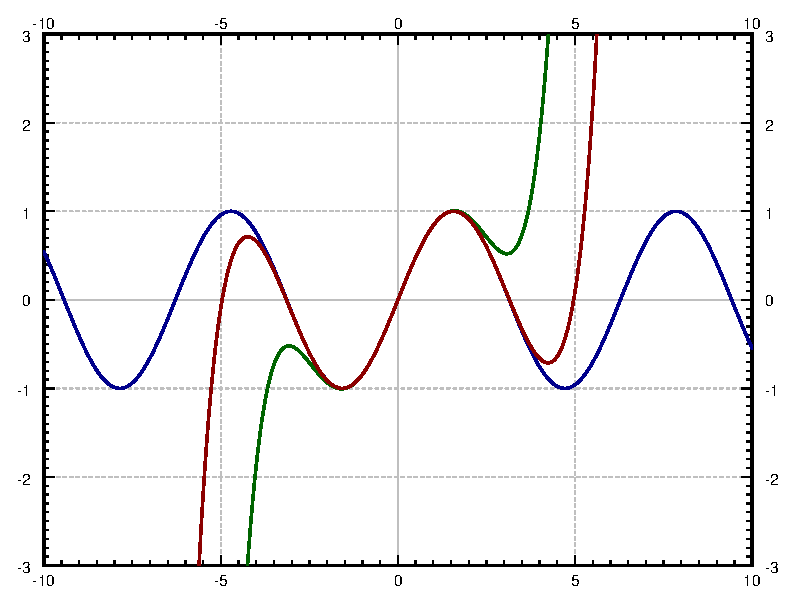
\includegraphics[width=2.6in]{../figures/ps-sin}

\vspace*{-70pt}

On the plot is sine, and the truncations

(partial sums) of degree 5 and 9.

\pause
\medskip

The approximation is good near $0$,

but gets worse further away.

\pause

It is better the more terms we take.

\end{frame}

\begin{frame}

We differentiate power series term-by-term like polynomials.

\medskip

$
\displaystyle
\frac{d}{dx}
\Biggl[\sum_{k=0}^\infty a_k {(x-x_0)}^k\Biggr]
=
\frac{d}{dx}
\Biggl[
a_0
+ a_1 (x-x_0)
+ a_2 {(x-x_0)}^2
+ a_3 {(x-x_0)}^{3}
+ \cdots
\Biggr]
$

\pause
$
\displaystyle
\phantom{
\frac{d}{dx}
\Biggl[\sum_{k=0}^\infty a_k {(x-x_0)}^k\Biggr]
}
=
a_1
+ 2 a_2 (x-x_0)
+ 3 a_3 {(x-x_0)}^{2}
+ \cdots
\pause
=
\sum_{k=1}^\infty k a_k {(x-x_0)}^{k-1}
$

\pause
\medskip

Radius of convergence is the same.
\pause
\quad
Notice how $a_0$ disappeared.

\pause
\medskip

\textbf{Example:}
Let $\displaystyle y = e^x = 
\sum_{k=0}^\infty \frac{1}{k!} x^k$.
\quad
\pause
Compute
\quad
$\displaystyle
y' = \sum_{k=1}^\infty k \frac{1}{k!} x^{k-1}
\pause
=
\sum_{k=1}^\infty \frac{1}{(k-1)!} x^{k-1}$

\pause
\medskip

Reindex (replace $k$ with $k+1$):
\quad
$\displaystyle
\sum_{k=1}^\infty \frac{1}{(k-1)!} x^{k-1} =
\sum_{k+1=1}^\infty \frac{1}{\bigl((k+1)-1\bigr)!} x^{(k+1)-1}
\pause
=
\sum_{k=0}^\infty \frac{1}{k!} x^k$.

\pause
\medskip

Notice that $y' = y$ (we knew that of course).

\end{frame}

\begin{frame}
Power series can be added:
\[
\left(\sum_{k=0}^\infty a_k {(x-x_0)}^k\right)
+
\left(\sum_{k=0}^\infty b_k {(x-x_0)}^k\right)
=
\sum_{k=0}^\infty (a_k+b_k) {(x-x_0)}^k .
\]
\pause
Multiplied:
\[
\alpha
\left(\sum_{k=0}^\infty a_k {(x-x_0)}^k\right)
=
\sum_{k=0}^\infty \alpha a_k {(x-x_0)}^k .
\]
\pause
and
\[
\left(\sum_{k=0}^\infty a_k {(x-x_0)}^k\right)
\,
\left(\sum_{k=0}^\infty b_k {(x-x_0)}^k\right)
=
\sum_{k=0}^\infty c_k {(x-x_0)}^k ,
\]
where
$c_k = a_0b_k + a_1 b_{k-1} + \cdots + a_k b_0$.

\pause
\medskip

The radius of convergence 
is at least the minimum of the radii of the two series.

\pause
\medskip

\textbf{Example:}
\quad
$\displaystyle \sum_{k=0}^\infty 2^k x^k + 
\sum_{k=0}^\infty (k+1) x^k = 
\sum_{k=0}^\infty (2^k + k + 1) x^k$

\end{frame}

\begin{frame}
Polynomials are finite power series:
$a_k$ are zero for all $k$ large enough.

\pause
\medskip

\textbf{Example:}

\quad
$2x^2-3x+4 = 4 + (-3)x + 2 x^2$,
\quad
$x_0 = 0$, 
$a_0 = 4$, $a_1 = -3$, $a_2 = 2$, and $a_k = 0$ for $k \geq 3$.

\pause
\medskip

Or for $x_0 = 1$:

\medskip

\quad
$2x^2-3x+4 = 3 + (x-1) + 2{(x-1)}^2$,
\quad
%$x_0 = 1$, 
$a_0 = 3$, $a_1 = 1$, $a_2 = 2$, and $a_k = 0$ for $k \geq 3$.

\medskip

\pause
How to do it? \pause Write
\quad
$2x^2-3x+4 = a_0 + a_1 (x-1) + a_2 {(x-1)}^2$,
\quad
expand and solve.

\pause
\medskip

You could also use Taylor's formula:

\medskip

If $f(x) = 2x^2-3x+4$, then
$f'(x) = 4x-3$, and $f''(x) = 4$.

So $a_0 = f(1) = 3$, $a_1 = f'(1) = 1$, $a_2 = \frac{f''(1)}{2} = 2$

\end{frame}

\begin{frame}
\uncover<+->{%
\emph{Geometric series}:
\quad
$\displaystyle
\sum_{k=0}^\infty x^k =
1 + x + x^2 + \cdots
=
\frac{1}{1-x}
\quad
\text{for }
-1 < x < 1 $.}

\uncover<+->{%
Radius of convergence is 1.
The series diverges
when $x \leq -1$ and $x \geq 1$,}

\uncover<+->{%
but $\dfrac{1}{1-x}$ is defined for all $x \neq 1$.}

\medskip

\uncover<+->{%
We can expand any rational function $\frac{p(x)}{q(x)}$ around
any point $x_0$ as long as $q(x_0) \neq 0$.}

\medskip

\uncover<+->{%
\textbf{Example:}
Expand $\frac{x}{1+2x+x^2}$ around $x_0 = 0$ and find $\rho$.}

\medskip

%First $1+2x+x^2 = {(1+x)}^2 = {\bigl(1-(-x)\bigr)}^2$.
\quad
$\displaystyle
\uncover<+->{%
\frac{x}{1+2x+x^2}
=
x \,
{\left(
\frac{1}{1-(-x)}
\right)}^2
}
\uncover<+->{%
=
x \,
{ \left( 
\sum_{k=0}^\infty {(-1)}^k x^k 
\right)}^2
}
\uncover<+->{%
=
x \,
\left(
\sum_{k=0}^\infty c_k x^k 
\right)
}
\uncover<+->{%
=
\sum_{k=0}^\infty c_k x^{k+1}
,}
$

\quad
\uncover<.(-1)->{%
$c_0 = 1$, $c_1 = -1 -1 = -2$, $c_2 = 1+1+1 = 3$, etc.
(as per product formula)}

\medskip

\uncover<+->{%
So\quad
$\displaystyle
\frac{x}{1+2x+x^2}
=
\sum_{k=1}^\infty {(-1)}^{k+1} k x^k
= x-2x^2+3x^3-4x^4+\cdots$
}

\medskip

\uncover<+->{%
$\rho$ is at least 1 as the series we used had $\rho=1$.}

\uncover<+->{%
Ratio test confirms $\rho=1$:
\quad
$\displaystyle
\lim_{k\to\infty}
\left\lvert \frac{a_{k+1}}{a_k} \right\rvert
=
\lim_{k\to\infty}
\left\lvert \frac{{(-1)}^{k+2} (k+1)}{{(-1)}^{k+1}k} \right\rvert
=
\lim_{k\to\infty}
\frac{k+1}{k}
= 1 .
$
}

\end{frame}

\begin{frame}
We can use partial fractions:

\pause
\medskip

\textbf{Example:}

\quad
$\displaystyle
\frac{x^3+x}{x^2-1}
=
x + \frac{1}{1+x} - \frac{1}{1-x}
\pause
=
x + \sum_{k=0}^\infty {(-1)}^k x^k - \sum_{k=0}^\infty x^k
\pause
=
- x + \sum_{\substack{k=3 \\ k \text{ odd}}}^\infty (-2) x^k
\pause
=
- x + \sum_{n=1}^\infty (-2) x^{2n+1}
$.

\pause
$\rho=1$ here.

\pause
\medskip

We may have to use algebra:

\pause
\medskip

\textbf{Example:}
Expand $\dfrac{1}{x}$ around $x_0 = 7$.

\pause
\medskip

\quad
$\displaystyle
\frac{1}{x}
=
\frac{1}{7 - (x-7)}
\pause
=
\frac{1}{7}
\frac{1}{1 - \frac{1}{7}(x-7)}
\pause
=
\frac{1}{7}
\sum_{k=0}^\infty {\left(\frac{1}{7}(x-7) \right)}^k
\pause
=
\sum_{k=0}^\infty \frac{1}{7^{k+1}} (x-7)^k$.

\pause
\medskip

Converges when 
$\left\lvert \dfrac{1}{7}(x-7) \right\rvert < 1$ or
$\lvert x-7 \rvert < 7$, so $\rho = 7$.


\end{frame}

\end{document}
